% Options for packages loaded elsewhere
\PassOptionsToPackage{unicode}{hyperref}
\PassOptionsToPackage{hyphens}{url}
%
\documentclass[
]{article}
\usepackage{amsmath,amssymb}
\usepackage{iftex}
\ifPDFTeX
  \usepackage[T1]{fontenc}
  \usepackage[utf8]{inputenc}
  \usepackage{textcomp} % provide euro and other symbols
\else % if luatex or xetex
  \usepackage{unicode-math} % this also loads fontspec
  \defaultfontfeatures{Scale=MatchLowercase}
  \defaultfontfeatures[\rmfamily]{Ligatures=TeX,Scale=1}
\fi
\usepackage{lmodern}
\ifPDFTeX\else
  % xetex/luatex font selection
\fi
% Use upquote if available, for straight quotes in verbatim environments
\IfFileExists{upquote.sty}{\usepackage{upquote}}{}
\IfFileExists{microtype.sty}{% use microtype if available
  \usepackage[]{microtype}
  \UseMicrotypeSet[protrusion]{basicmath} % disable protrusion for tt fonts
}{}
\makeatletter
\@ifundefined{KOMAClassName}{% if non-KOMA class
  \IfFileExists{parskip.sty}{%
    \usepackage{parskip}
  }{% else
    \setlength{\parindent}{0pt}
    \setlength{\parskip}{6pt plus 2pt minus 1pt}}
}{% if KOMA class
  \KOMAoptions{parskip=half}}
\makeatother
\usepackage{xcolor}
\usepackage[margin=1in]{geometry}
\usepackage{longtable,booktabs,array}
\usepackage{calc} % for calculating minipage widths
% Correct order of tables after \paragraph or \subparagraph
\usepackage{etoolbox}
\makeatletter
\patchcmd\longtable{\par}{\if@noskipsec\mbox{}\fi\par}{}{}
\makeatother
% Allow footnotes in longtable head/foot
\IfFileExists{footnotehyper.sty}{\usepackage{footnotehyper}}{\usepackage{footnote}}
\makesavenoteenv{longtable}
\usepackage{graphicx}
\makeatletter
\def\maxwidth{\ifdim\Gin@nat@width>\linewidth\linewidth\else\Gin@nat@width\fi}
\def\maxheight{\ifdim\Gin@nat@height>\textheight\textheight\else\Gin@nat@height\fi}
\makeatother
% Scale images if necessary, so that they will not overflow the page
% margins by default, and it is still possible to overwrite the defaults
% using explicit options in \includegraphics[width, height, ...]{}
\setkeys{Gin}{width=\maxwidth,height=\maxheight,keepaspectratio}
% Set default figure placement to htbp
\makeatletter
\def\fps@figure{htbp}
\makeatother
\setlength{\emergencystretch}{3em} % prevent overfull lines
\providecommand{\tightlist}{%
  \setlength{\itemsep}{0pt}\setlength{\parskip}{0pt}}
\setcounter{secnumdepth}{-\maxdimen} % remove section numbering
\ifLuaTeX
  \usepackage{selnolig}  % disable illegal ligatures
\fi
\usepackage{bookmark}
\IfFileExists{xurl.sty}{\usepackage{xurl}}{} % add URL line breaks if available
\urlstyle{same}
\hypersetup{
  pdftitle={Project\_Data583\_Exploratory analysis},
  pdfauthor={Baldeep Dhada, Han Chen, Somya Nagar},
  hidelinks,
  pdfcreator={LaTeX via pandoc}}

\title{Project\_Data583\_Exploratory analysis}
\author{Baldeep Dhada, Han Chen, Somya Nagar}
\date{2024-03-05}

\begin{document}
\maketitle

\subsubsection{Instroduce about dataset}\label{instroduce-about-dataset}

\paragraph{Summary}\label{summary}

This data set comprises the medical histories of 299 patients diagnosed
with heart failure, and the target variable is \texttt{death\_event}with
each patient's profile containing 12 clinical attributes.

\begin{longtable}[]{@{}
  >{\raggedright\arraybackslash}p{(\columnwidth - 6\tabcolsep) * \real{0.2466}}
  >{\raggedright\arraybackslash}p{(\columnwidth - 6\tabcolsep) * \real{0.2466}}
  >{\raggedright\arraybackslash}p{(\columnwidth - 6\tabcolsep) * \real{0.2603}}
  >{\raggedright\arraybackslash}p{(\columnwidth - 6\tabcolsep) * \real{0.2466}}@{}}
\toprule\noalign{}
\begin{minipage}[b]{\linewidth}\raggedright
variables
\end{minipage} & \begin{minipage}[b]{\linewidth}\raggedright
Type
\end{minipage} & \begin{minipage}[b]{\linewidth}\raggedright
description
\end{minipage} & \begin{minipage}[b]{\linewidth}\raggedright
values
\end{minipage} \\
\midrule\noalign{}
\endhead
\bottomrule\noalign{}
\endlastfoot
age & Integer & age of the patient (years) & {[}40,95{]} \\
anaemia & Binary & decrease of red blood cells or hemoglobin & 0,1 \\
creatinine\_phosphokinase & Integer & level of the CPK enzyme in the
blood(mcg/L) & {[}23,7861{]} \\
diabetes & Binary & if the patient has diabetes & 0,1 \\
ejection\_fraction & Integer & percentage of blood leaving the heart at
each contraction (\%) & {[}14,80{]} \\
high\_blood\_pressure & Binary & if the patient has hypertension &
0,1 \\
platelets & Continuous & platelets in the blood(kiloplatelets/mL) &
{[}25100,850000{]} \\
serum\_creatinine & Continuous & level of serum creatinine in the blood
(mg/dL) & {[}0.5,9.4{]} \\
serum\_sodium & Integer & level of serum sodium in the blood (mEq/L) &
{[}113,148{]} \\
sex & Binary & woman or man & 0,1 \\
smoking & Binary & if the patient smokes or not & 0,1 \\
time & Integer & follow-up period (days) & {[}4,285{]} \\
death\_event & Binary & if the patient died during the follow-up period
& 0,1 \\
\end{longtable}

\paragraph{statistically descriptive
analysis}\label{statistically-descriptive-analysis}

Target: As the pie plot shows below, our targeted variables
\texttt{death\_event} is unbalance with more survival observation than
the dead one.

\includegraphics[width=4in,height=\textheight]{images/visualization (5).png}

Quantitative Variables: we visualize 7 quantitative variables with
histogram and fit each distribution of them, except `time` which has two
peaks. The upper four plots comply to gamma distribution and the below
to follow normal distribution:

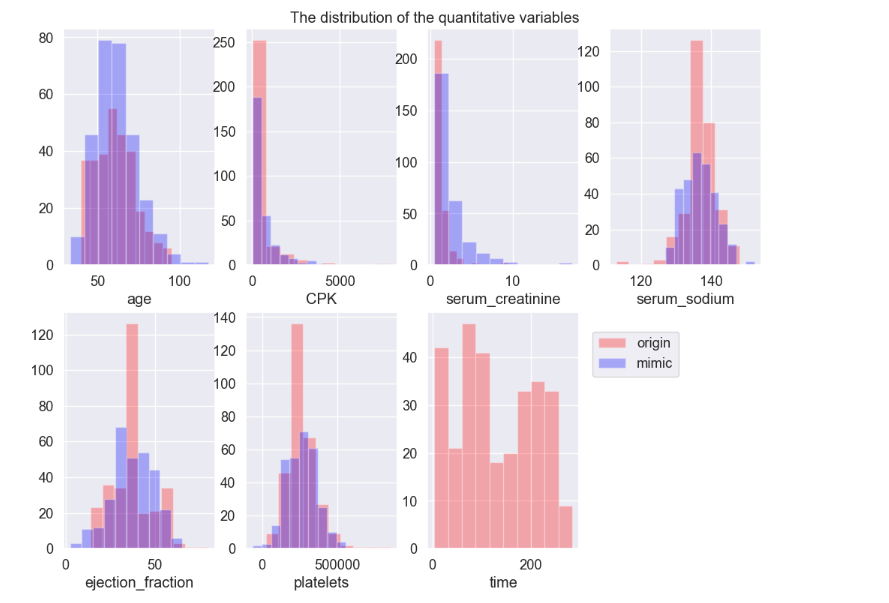
\includegraphics{quantitative distribution.png}

\begin{figure}
\centering
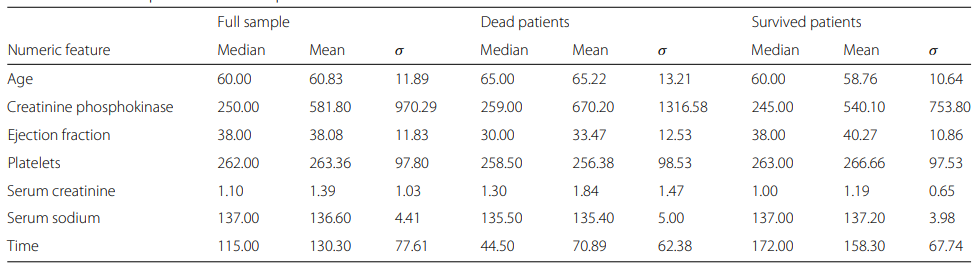
\includegraphics{table.png}
\caption{Statistical quantitative description of the numeric features}
\end{figure}

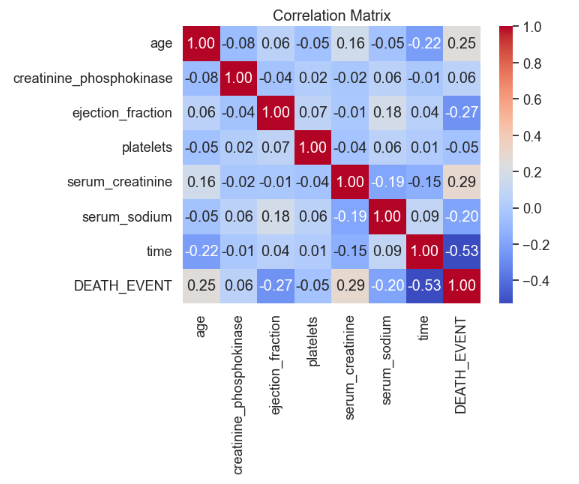
\includegraphics{correlative matrix.png}

\end{document}
